\documentclass[a4paper,11pt]{article}
\usepackage[polish]{babel}
\usepackage[utf8]{inputenc}
\usepackage[T1]{fontenc}
\usepackage{graphicx}
\usepackage{anysize}
\usepackage{enumerate}
\usepackage{times}
\usepackage{subfig}

%\marginsize{left}{right}{top}{bottom} %\mbox{ } nie lam linii, hspace{ }
\marginsize{3cm}{3cm}{3cm}{3cm}
\sloppy

\begin{document}

\section*{Techniki cyfrowe -- wprowadzenie}

\emph{Sygnałami cyfrowymi} nazywamy dwuwartościowe sygnały dyskretne. Są one odporne na zakłócenia i~mogą być przekazywane z~dużą szybkością i~niezawodnością. \emph{Technika cyfrowa} jest to dziedzina nauki i~techniki związana z~przetwarzaniem sygnałów cyfrowych. Układy i~systemy, w~których zachodzi przetwarzanie sygnałów cyfrowych nazywamy \emph{układami} i~\emph{systemami cyfrowymi} (digital circuits, digital systems).


Pierwsze układy cyfrowe były układami przekaźnikowymi, a~ich opis i~metody projektowania wykorzystywały algebrę Boole'a. w~algebrze Boole'a są trzy działania na argumentach zerojedynkowych: suma logiczna (alternatywa zdarzeń), iloczyn logiczny (koniunkcja zdarzeń) i~inwersja (negacja). Za pomocą takich działań można określać różne funkcje, a~biorąc zestaw przekaźników można zbudować układ cyfrowy realizujący daną funkcję. Przekaźnik działa w~taki sposób, że jeśli w~jego uzwojeniu płynie prąd, to jego styki są w~jednym z~dwóch położeń: mogą być zwarte albo rozwarte. Na rysunku \ref{fig:ukladPrzekaznikowy} pokazano jak w~oparciu o~dwa przekaźniki można zrealizować sumę logiczną. Połączenie punktu A i~B następuje, gdy styk choć jednego z~dwóch przekaźników jest zwarty.


\begin{figure}[!htb]
\centerline{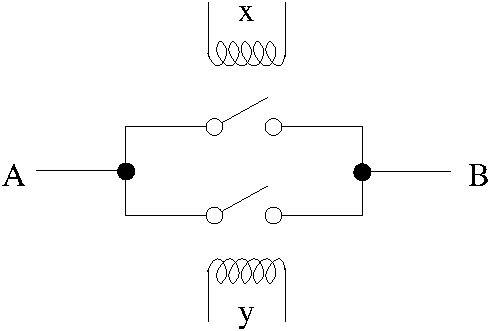
\includegraphics[scale=0.6]{uklad-przekaznikowy.pdf}}
\caption{Układ przekaźnikowy – suma logiczna}
\label{fig:ukladPrzekaznikowy}
\end{figure}


Układy zbudowane z~elementów przekaźnikowych nazywane są układami przełączającymi (ang. switching circuits).  W~latach 30. zbudowano komputer za pomocą przekaźników. Była to pierwsza maszyna obliczeniowa MARK~I~zbudowana przez Howarda Aikena. Późniejszy rozwój elektroniki pozwolił na budowanie bezstykowych układów cyfrowych. Wykorzystywano do tego celu lampy elektronowe, tranzystory, układy magnetyczne itp. Układy cyfrowe zbudowane z~takich elementów nazwano \emph{bramkami logicznymi}. Zastosowanie bramek do budowy układów cyfrowych spowodowało szybki rozwój komputerów, układów automatyki i~elektroniki profesjonalnej

W~jednym \emph{układzie scalonym} już w~latach 60. można było pomieścić kilka bramek, a~co ważniejsze pobierana moc była znacznie mniejsza od mocy pobieranej przez bramki budowane z~elementów dyskretnych. Te pierwsze układy scalone, tzw. \emph{małej skali integracji} SSI (small scale integration) spowodowały rozpowszechnienie techniki cyfrowej w~wielu dziedzinach zastosowań. Od tej pory aż do dnia dzisiejszego trwa nieustanny rozwój technologii układów scalonych. Powstały układy \emph{średniej skali integracji} MSI (medium scale integration), a~następnie \emph{wielkiej skali integracji} LSI (large scale integration). Współcześnie stosuje się układy \emph{bardzo wielkiej skali integracji} VLSI (very large scale integration). Projektanci układów cyfrowych wykonują złożone projekty wykorzystując jeden układ scalony, jak np. programowaną matrycę logiczną. Stosują przy tym bardzo zaawansowane metody komputerowego wspomagania projektowania CAD.

\begin{figure}[!htb]
\centerline{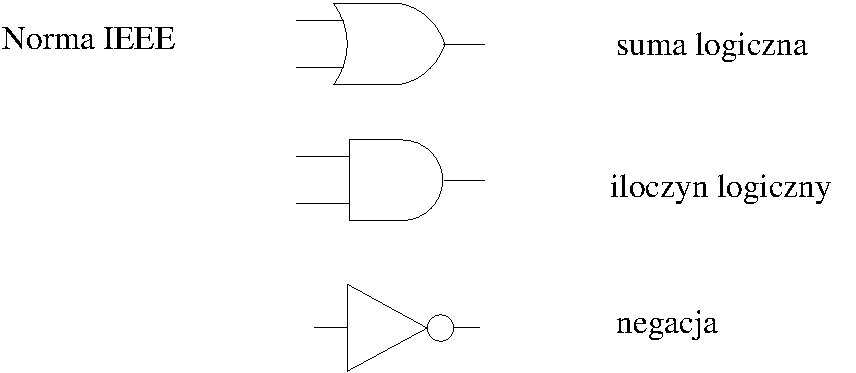
\includegraphics[scale=0.6]{symbole-bramek.pdf}}
\caption{Symbole bramek logicznych}
\label{fig:symboleBramekLogicznych}
\end{figure}

Układ scalony (integrated circuit, chip, potocznie kość) jest to zminiaturyzowany układ elektroniczny zawierający w~swym wnętrzu od kilku do setek milionów podstawowych elementów elektronicznych, takich jak tranzystory, diody, rezystory, kondensatory. Zwykle jest on zamknięty w~hermetycznej obudowie -- szklanej, metalowej, ceramicznej lub wykonanej z~tworzywa sztucznego.\\
\begin{figure}[!htb]
\centering
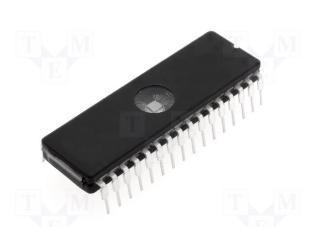
\includegraphics[width=0.3\textwidth]{uklad1.jpg}
\quad
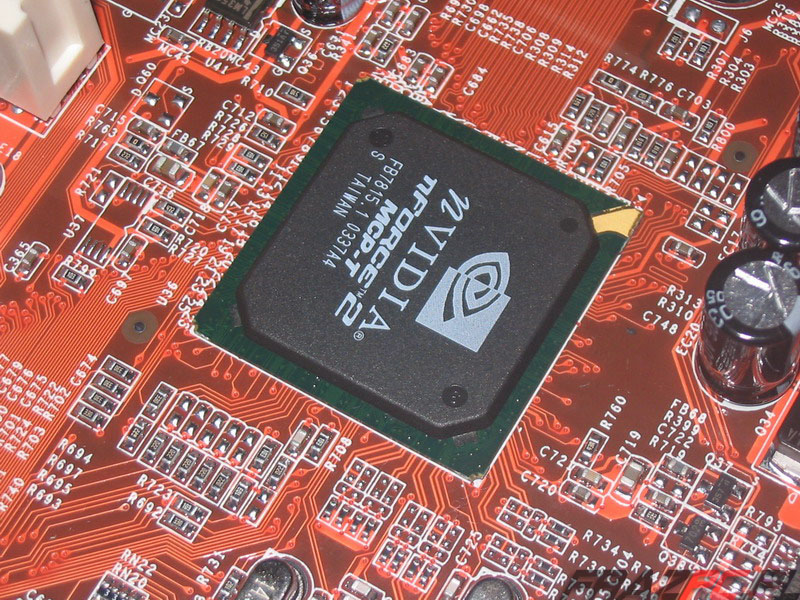
\includegraphics[width=0.3\textwidth]{uklad2.jpg}
\quad
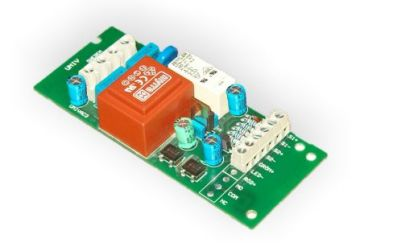
\includegraphics[width=0.3\textwidth]{uklad3.jpg}
\caption{Układy scalone}
\label{fig:ukladyScalone}
\end{figure}\\
Ze względu na sposób wykonania układy scalone dzieli się na główne grupy:
\begin{itemize}
\item monolityczne, w~których wszystkie elementy, zarówno elementy czynne jaki~bierne, wykonane są w~monokrystalicznej strukturze półprzewodnika;
\item hybrydowe na płytki wykonane z~izolatora nanoszone są warstwy przewodnika oraz materiału rezystywnego (zadaniem warstwy rezystywnej jest osłonięcie materiału podłoża przed działaniem czynników trawiących), które następnie są wytrawiane, tworząc układ połączeń elektrycznych oraz rezystory. Do tak utworzonych połączeń dołącza się indywidualne, miniaturowe elementy elektroniczne (w tym układy monolityczne). Ze względu na grubość warstw rozróżnia się układy cienkowarstwowe (warstwy ok. 2 mikrometrów)i~grubowarstwowe (warstwy od 5 do 50 mikrometrów)
\end{itemize}

Większość stosowanych obecnie układów scalonych jest wykonana w~technologii monolitycznej. Ponieważ w~układach monolitycznych praktycznie wszystkie elementy wykonuje się jako tranzystory, odpowiednio tylko przyłączając ich końcówki, dlatego też często mówi się o~gęstości upakowania tranzystorów na \emph{$mm^{2}$}.

Pierwsze elementy które można uznać za układ scalony, wyprodukowała już pod koniec lat 20. XX wieku firma Loewe. Była to lampa próżniowa zawierająca wewnątrz jednej bańki trzy triody (dwie sygnałowei~jedną głośnikową), dwa kondensatoryi~cztery rezystory, całość była przeznaczona do pracy jako jednoobwodowy radioodbiornik reakcyjny. Jednak dopiero w~1958 opracowałi~skonstruował układ scalony Jack Kilby, za co otrzymał Nagrodę Nobla z~fizyki w~roku 2000. \\

\emph{Tranzystor} jest to trójzłączowy półprzewodnikowy element elektroniczny, posiadający zdolność wzmacniania sygnału elektrycznego.

Pierwszy tranzystor skonstruowano w~1947 roku w~laboratoriach firmy Bell Telephone Laboratories. Wynalazcami są John Bardeen, Walter Houser Brattain oraz William Bradford Shockley, za co otrzymali Nagrodę Nobla z~fizyki w~1956. Wynalezienie tranzystora uważa się za przełom w~elektronice, zastąpił on bowiem duże, zawodne lampy elektronowe, dając początek coraz większej miniaturyzacji przyrządówurządzeń elektronicznych. 

Tranzystor ze względu na swoje właściwości wzmacniające jest  wykorzystywany do budowy wzmacniaczy różnego rodzaju, a~także jest kluczowym elementem w~konstrukcji wielu układów elektronicznych, takich jak źródła prądowe, lustra prądowe, stabilizatory, przesuwniki napięcia, klucze elektroniczne, przerzutniki, czy generatory. z~tranzystorów buduje się także bramki logiczne realizujące podstawowe funkcje boolowskie. Są one także podstawowym budulcem wszelkiego rodzaju pamięci półprzewodnikowych (RAM, ROM, itd.).

W roku 2001 holenderscy naukowcy z~Uniwersytetu w~Delft stworzyli tranzystor składający się z~jednej cząsteczki. Rozmiar tego cudu miniaturyzacji wynosi zaledwie jeden nanometr ($10^{-9}m$), a~do zmiany swojego stanu (włączony/wyłączony) potrzebuje on tylko jednego elektronu. Naukowcy przewidują, że ich wynalazek pozwoli na konstruowanie układów miliony razy szybszych od obecnie stosowanych, przy czym ich wielkość pozwoli na dalszą miniaturyzację elektronicznych urządzeń.
\end{document}
